\documentclass{article}
\usepackage[utf8]{inputenc}
\usepackage[margin=0.625in]{geometry}
\usepackage{parskip, setspace}
\setstretch{1.5}
\usepackage{amsmath, amsfonts}
%\numberwithin{equation}{subsection}
\usepackage{graphicx, caption, wrapfig}
\usepackage{hyperref}
\usepackage{multirow}

\usepackage{biblatex}
\addbibresource{bib.bib}

\renewcommand{\arraystretch}{1.5}

\title{\Large \vspace{-0.625in} CS 530: High-Performance Computing \\ Benchmarking Matrix Multiplication in Fortran vs Python \vspace{-0.35in}}
\author{Nathan Chapman \vspace{-0.15in} \\ {\normalsize Central Washington University}}
\date{\normalsize \vspace{-0.15in}\today}

\begin{document}

\maketitle

    % \begin{center}
    % Abstract \\
    
    % \end{center}

\tableofcontents

% \pagebreak

\section{Introduction}

    There has always been what's known in computer science as ``the two language problem''.  This describes the discepancy between programming languages that are ``hard'' or take a long time to write but execute extremely quickly, and those that are ``easy'' or take little time to write but take much more time than the former.  When it comes to high-performance computing, the former is neccessary not only for reducing the run-time but also for those languages ability to interface more directly with hardware.  While Assembly would be the ultimate in terms of speed, using it to to write complex procedures, especially for scientific workloads, is unreasonable for the vast majority of people and specifically scientists.  The two-language problem and the need for high-performance languages leads us to compare the efficiencies of languages in each category: Fortran and Python.

    Fortran (named for ``Formula Translating System'') was created in the very beginning of the computing age to help in writing procedures for scientitic computing.  As such, it has been one of the main choices of implementation for high-perforamnce computational scientists across the world.  Fortran's curation for numerical computing and native support for arrays (of any dimension) and other mathematical and scientific procedures still makes it a top choice even for 2024.  That being said, there's a lot that needs to go into using Fortran to get from a scientific idea to a number;  that's where other languages such as Python come in.
\pagebreak
    Python has exploded in recent years in the computational science due to how easy it is to write.  Python is so easy to use and write that it is the de-facto standard of languages to use in teaching those new to programming and computer science.  Part of this ease comes from not needing to manually compile source code into binaries; this is instead done through ``interpretation''.  It's exactly because of these though that make it execute its procedures relatively slowly compared to languages like Fortran and C and C++.  One such example, to highlight their differences in execution time, is matrix multiplication.

\section{Methods}

    The mathematical definition of matrix multiplication takes the form

    \begin{equation} \label{eq:matrix_power}
        (A B)_{i,j} = \sum_{k = 1}^{L} A_{ik} B_{kj}
    \end{equation}

    where $A,B$ are $N \times L$ and $L \times M$ matrices, respectively, and $(A B)_{i,j}$ is the element of the $i$-th row and $j$-th column of the product.  Because this definition is for $N$ rows, $M$ columns, and $L$ elements in the sum, the total number of either additions or multiplications is $N \times M \times L$.  For the multiplication of an $N \times N$ square matrix with itself (a ``matrix power''), this leads to $N^3$ operations for a single multiplication.  If this is done multiple times $p$ to create an arbitrary matrix power $A^p$ of an $N \times N$ matrix $A$, the number of total operations needed is $p N^3$.  Using asymptotic notation, this means that matrix powers are $\mathcal{O}(p N^3)$.

    In order to test the efficiencies of the Fortran and Python implementations, such matrices need to be initialized.  For this investigation, these matrices were initialized using random numbers.  The default psuedo-random number generator in Fortran is xoshiro256**.  Similarily, the default psuedo-random number generator in Python is Mersenne Twister.  All elements of the initial matrices are between 0 and 1; negative numbers could also be used to mitigate overflow in their data-types as the elements of the matrix-product grow astronomically large.

\section{Results}

    Figures \ref{fig:dimension} and \ref{fig:power} show timings for the Fortran and Python implementations of matrix power algorithm as defined in equation \ref{eq:matrix_power} scanning over dimension and power respectively. Furthermore, timings were taken using Fortran's \verb|time8| instrinsic function (other timing functions and subroutines such as \verb|mclock, cpu_time, etime| were used but did not give significant results) and matrix elements are represented with 128-bit floating point numbers.  Benchmarking results were generated on a machine with specifications show in table \ref{tbl:specs}.  Futher details on software versioning to be used for reproducibility is found in table \ref{tbl:versions}.

    \begin{figure}[h]
        \centering
        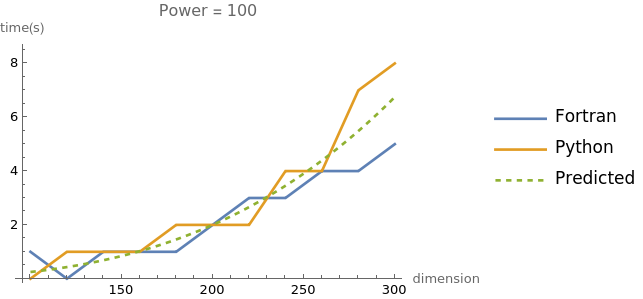
\includegraphics[width=0.66\textwidth]{images/dimension.png}
        \caption{Comparison of timings over differing dimensions with constant power}
        \label{fig:dimension}
    \end{figure}

    \begin{figure}[h]
        \centering
        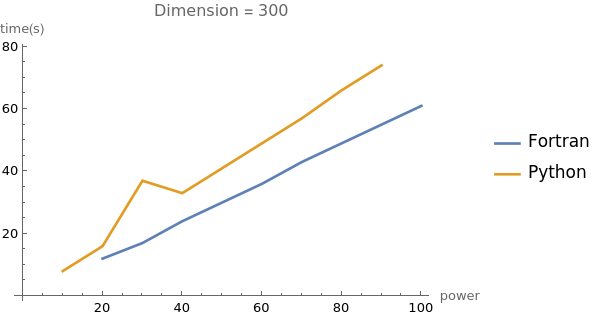
\includegraphics[width=0.66\textwidth]{images/power.png}
        \caption{Comparison of timings over constant dimension with differing powers}
        \label{fig:power}
    \end{figure}

    \begin{table}[h]
        \centering
        \begin{tabular}{|c|c|}
            \hline
            Operating System & Manjaro Linux \\
            \hline
            Kernel Version & 6.6.26-1-MANJARO (64-bit) \\
            \hline
            Processors & 24 × 13th Gen Intel® Core™ i7-13700K \\
            \hline
            Memory & 31.2 GiB of RAM \\
            \hline
            Graphics Processor & NVIDIA GeForce RTX 3060 Ti/PCIe/SSE2 \\
            \hline
            Manufacturer & ASRock \\
            \hline
            Product Name & B760M Steel Legend WiFi \\
            \hline
        \end{tabular}
        \caption{Specifications of benchmarking machine}
        \label{tbl:specs}
    \end{table}

    \begin{table}[h]
        \centering
        \begin{tabular}[pos]{|c|c|}
            \hline
            Fortran Compiler & GNU Fortran (GCC) 13.2.1 20230801 \\
            \hline
            Build Platform  & cmake version 3.28.3, GNU Make 4.4.1 \\
            \hline
            Scripting lang  & Python 3.11.8 \\
            \hline
        \end{tabular}
        \caption{Software versions used in eenchmarking}
        \label{tbl:versions}
    \end{table}
\pagebreak
\section{Discussion}

    Theory tells us that Fortran should be much quicker than Python, especially for large matrices and/or large powers.  Figure \ref{fig:dimension} highlights this to be true in practice.  While the trend in \ref{fig:dimension} agrees with theory, there are minor discrepancies as the timings show that there are in fact cases where Python actually exectues in \emph{less} time than Fortran.  These results are surprising and the cause could be investigated in later research.  For the data gathered, a nonlinear trend can be seen in figure \ref{fig:dimension} which qualitatively agrees with the prediction (in figure \ref{fig:dimension} show by $2.5 \times 10^{-9} * p N^3$ ) that the execution time of the multiplication should follow $p N^3$.

    Figure \ref{fig:power} is consistent with our hypothesis and theoretical prediction as Fortran is always faster than Python; the difference between them growing as the power increases.  For the data gathered, the data and trends also agree with our prediction that the execution time should increases linearly with power since the number of constant-time operations is $p N^3$.
\pagebreak
\section{Conclusion}

    While Python is an excellent resource to use in many situtaions, the performance of languages like Fortran and C/C++ cannot be beat.  Additionally, Fortran and C/C++ include the ability to interface with graphics processing units through the CUDA platform, enabling massively parallel computation for even further reduction in execution time and increase in problem size.

\end{document}